\documentclass[11pt,english,french]{scrreprt}
\usepackage{lmodern}
\usepackage{babel}
\renewcommand{\familydefault}{\rmdefault}
\usepackage[T1]{fontenc}
\usepackage{ucs}
\usepackage[utf8x]{inputenc}
\usepackage[a4paper]{geometry}
\geometry{verbose,tmargin=2cm,bmargin=2cm,lmargin=2cm,rmargin=2cm,headheight=2cm,footskip=1cm}
\setlength{\parskip}{\smallskipamount}
\setlength{\parindent}{0pt}

\usepackage{amsthm}
\usepackage{booktabs}
\usepackage{amsmath}
\usepackage[unicode=true, pdfusetitle,
 bookmarks=true,bookmarksnumbered=false,bookmarksopen=false,
 breaklinks=false,pdfborder={0 0 1},backref=false,colorlinks=false]
 {hyperref}

\makeatletter
\usepackage{colortbl}
\usepackage{color}
\usepackage[dvipsnames]{xcolor}
\usepackage{wrapfig}
\usepackage{graphicx}
\usepackage{listings}
\usepackage[calcwidth]{titlesec}
\usepackage{fix-cm}
\usepackage{multicol}
\usepackage{verbatim}
\usepackage{moreverb}
\usepackage{nicefrac}
\usepackage{amssymb}
\usepackage{array}
\usepackage{tabularx}
\usepackage{subfig}

\theoremstyle{remark}
  \newtheorem*{rem*}{Remarque}
\theoremstyle{definition}
  \newtheorem*{defi}{Définition}
  \newtheorem{ques}{Question}[section]

\definecolor{MyDarkBlue}{rgb}{0,0.08,0.45}

\lstset{language=C,
	 	basicstyle=\small\ttfamily,
		keywordstyle=\small\ttfamily,
		identifierstyle=,
		commentstyle=\textcolor{OliveGreen},
		columns=fullflexible,
		stringstyle=\small\ttfamily,
		showstringspaces=false,numberstyle=\tiny, breaklines=false, tabsize=4}

\titleformat{\section}[hang]{\sffamily\bfseries}
 {\Large\thesection}{12pt}{\Large}[{\titlerule[0.5pt]}]

\def\thickhrulefill{\leavevmode \leaders \hrule height 1pt\hfill \kern \z@}
\renewcommand{\maketitle}{\begingroup%
    \let\footnotesize\small
    \let\footnoterule\relax
    \parindent \z@
    \reset@font
    \begin{flushleft}
      \huge \sffamily \bfseries\color{orange} \@title
    \end{flushleft}
    \hrule height 1pt
    \begin{flushright}
      \large\sffamily\color{MyDarkBlue}\@author
    \end{flushright}
  \endgroup%
  \setcounter{footnote}{0}%
}

\AtBeginDocument{
  \def\labelitemi{\normalfont\bfseries{--}}
}

\makeatletter
\renewcommand\thesection{\arabic{section}}
\@addtoreset{section}{chapter}
\makeatother

\makeatother
\begin{document}
	
\title{LI310 - Examen 2009 Rattrapage\\
Mardi 27 janvier 2010}
\author{Benjamin BARON}

\maketitle

\section{Signal} % (fold)

Signal porteur d'informations de fréquences strictement inférieures à 15 kHz.\\
Echantillon produit codé sur 16 bits (ie. $2^{16}$ niveaux de quantification).\\
Message numérique produit transmis en bande de base.

\begin{ques}
	Fréquence d'échantillonnage $f_e$ a utiliser pour minimiser le débit du message numérique produit à l'issue de l'opération de numérisation.
	
	Théorème d'échantillonnage de Shannon :\[f_e > 2f_{max}\]
	Application numérique ($f_{max} = 15$ kHz) :\[f_e > 2\times 15 = 30\;\textrm{kHz}\]
\end{ques}

\begin{ques}\label{ques:2}
	Capacité $C$ du canal de transmission pour permettre la transmission de ce message numérique.
	
	Puisque le signal transmis est échantillonné à une fréquence d'échantillonnage $f_e=30$ kHz, et que le signal numérique est composé d'échantillons codés sur $r = 16$ bits, alors le canal de transmission doit avoir une capacité $C=f_e\times r=30\,000\times 16=480$ kbit/s au minimum.
\end{ques}


\begin{ques}
	Câble de bande passante $[0,\,200\textrm{ kHz}]$.\\
	Rapport signal-à-bruit : $\nicefrac{S}{N}=18$ dB.
	
	D'après la loi de Shannon, la capacité maximale du canal considéré est exprimée par :\[C_{max}=B\log_2\left(1+\frac{P_S}{P_N}\right)\]
	Or \[\frac{P_S}{P_N}=10^{\frac{\nicefrac{S}{N}}{10}}= 10^{\frac{18}{10}}\approx 63,096\]
	Ainsi, on a :\[C_{max}=200.10^3\times \log_2(1+63,096)=1,20\;\textrm{Mbit/s}\]
	
	Puisque $C_{max}=1\,200\;\textrm{kbit/s}>C=480\;\textrm{kbit/s}$, alors la transmission est théoriquement possible sur ce canal.
\end{ques}

\begin{ques}
	Utilisation d'un code NRZ binaire ($M=2$) pour réaliser la transmission.
	
	D'après la loi de Nyquist :\[C \leqslant 2B\log_2(M) = 2\times 200.10^3\log_2(2) = 400\;\textrm{kbit/s}\]
	Or $C=480$ kbit/s, donc c'est impossible.
\end{ques}

\begin{ques}
	Utilisation d'un code NRZ-8 ($M=8$) pour réaliser la transmission.
	
	D'après la loi de Nyquist : \[C \leqslant 2B\log_2(M) = 2\times 200.10^3\log_2(8) = 1\,200\;\textrm{kbit/s} \leqslant C_{max}\]
	Or $C=480$ kbit/s, donc c'est possible.
\end{ques}

\begin{ques}
	La transmission à l'aide d'un signal NRZ-8 est optimale car avec celle-ci, on peut transmettre des messages à un débit maximal de $1\,200$ kbit/s (voir question précédente). Or la capacité maximale du canal considéré est également de $1\,200$ kbit/s.
	
	La liaison va alors fonctionner à un débit binaire de 480 kbit/s comme calculé à la question \ref{ques:2} (on n'envoie pas plus de données).
\end{ques}

\clearpage

\section{Réseaux locaux} % (fold)

\begin{ques}
	Réseau Ethernet à 1 Gbit/s, mode partagé, utilisation de CSMA/CD.\\
	Trame Ethernet > 64 octets ; vitesse de propagation du support : $t_{prop_{max}} = 5\;\mu$s/km. 
	
	Longueur maximum théorique d'un tel réseau. Contrainte lie à l'utilisation de CSMA/CD : \[t_{trans} > 2 t_{prop_{max}}\]
	Or \[t_{trans} > \frac{64\times 8}{1.10^9} > 0,512\;\mu\textrm{s} > 2 t_{prop_{max}} = 10\;\mu\textrm{s}\]
	On peut alors prolonger ce réseau sur $\nicefrac{0,512}{10}=51,2$ m.
\end{ques}

\begin{ques}
	Plusieurs segments d'un réseau local Ethernet sont reliés par des commutateurs afin de constituer un réseau maillé. Il faut utiliser le protocole \emph{Spanning Tree Protocole} dans les commutateurs : lorsque le switch reçoit une trame de S pour D, et qu'il ne sait pas sur quel LAN se situe D, il diffuse la trame sur tous ses ports, sauf celui sur lequel la trame lui est arrivée ; au passage, il note que pour joindre S, c'est le port d'arrivée de
	la trame qu'il faudra utiliser ; et ainsi de suite, jusqu'à ce qu'il reçoive une trame en provenance de D : à partir de ce moment, il saura quel est le port à utiliser pour réacheminer vers D.
	
	Un autre protocole, \emph{Source Routing} est utilisé à la place du \emph{Spanning Tree Protocol}. Ce protocole revient à identifier tous les chemins de la source vers une destination. Il faut effectivement modifier la trame Ethernet pour que ce protocole fonctionne : il faut ajouter un champ permettant à la source d'identifier le chemin à emprunter pour aller à la destination (\emph{Route Information}). Ce protocole est utilisé dans IEEE 802.5 (Token Ring).
\end{ques}

\begin{ques}
	Réseau local de l'entreprise commuté.\\
	Il n'existe plus de collisions : en utilisant la microsegmentation et le Full duplex, il n'existe pas de collisions entre terminaux car chaque terminal est relié directement à un commutateur.
	
	Le paramètre limitant la couverture géographique du réseau serait le type de câble utilisé pour relier les commutateurs aux terminaux, mais l'utilisation de répéteurs abolit cette contrainte de distance.

	Un hub est un répéteur multiport : chaque trame entrante est diffusée sur tous les ports sortants. Il n'y a donc pas de gestion du trafic qui passe au travers du hub. De ce fait, il y a des collisions qui amoindrissent les performances du réseau.\\
	Conclusion. Un réseau reposant sur des hubs sera moins performant qu'un réseau commuté.
\end{ques}

\begin{ques}
	Fonctions d'un noeud de transfert :\begin{itemize}
		\item Analyse et traduction de l'entête du paquet;
		\item Commutation ou routage;
		\item Multiplexage des paquets sur la sortie déterminée. 
	\end{itemize}
	
	Le temps de décision de commutation est le paramètre le plus critique en terme de traitement d'une trame dans un commutateur. Il est fonction de la taille de la table de commutation qui se trouve dans le commutateur.
	
	La vitesse de traitement d'un routeur est plus faible que celle d'un commutateur. Elle dépend également de la table de routage qui doit contenir l'emplacement de tous les destinataires pouvant passer par le même noeud.
\end{ques}

\begin{ques}
	Transport de la voix sur un réseau Ethernet.\\
	Il faut garantir un temps de transit au travers du réseau (SLA -- \emph{Service Level Agreement} négocié avec l'opérateur). En effet, ce temps de traversée doit être borné (< 250 - 200 ms dans le cas de la voix). Il faut alors utiliser une technique de priorité permettant aux trames prioritaires (ie. celles qui contiennent de la voix) de voir le réseau comme étant quasiment vide.
\end{ques}

\section{Routage} % (fold)

\begin{ques}
	Un routeur R1 possède les entrées suivantes dans sa table de routage : 
	
	\begin{tabularx}{\textwidth}{XXXll}
		\toprule 
		Adresse & Masque & Prochain saut & Interface & Métrique\tabularnewline
		\midrule
		\midrule 
		135.45.56.0 & 255.255.252.0/22 & {*} & eth0 & 0\tabularnewline
		\midrule 
		135.45.60.0 & 255.255.252.0/22 & {*} & eth1 & 0\tabularnewline
		\midrule 
		192.53.40.0 & 255.255.255.0/24 & 135.46.56.1 & \textbf{eth0} & 1\tabularnewline
		\midrule 
		192.57.36.0 & 255.255.255.0/24 & 135.46.59.1 & \textbf{eth0} & 1\tabularnewline
		\midrule 
		default & 0.0.0.0 & 135.46.63.254 & \textbf{eth1} & \tabularnewline
		\bottomrule
	\end{tabularx}
\end{ques}

\begin{ques}
	Pour chacune de ces adresses, que fera le routeur si un paquet avec cette adresse IP de destination lui parvient :\begin{itemize}
		\item 135.46.63.10 : routage direct sur interface eth1 (réseau d'adresse IP 135.46.60.0)
		\item 135.46.57.14 : routage direct sur interface eth0 (réseau d'adresse IP 135.46.56.0)
		\item 135.46.52.2 : routage indirect sur default -- eth1 (next hop 135.46.63.254)
		\item 192.53.40.7 : routage indirect sur interface eth0 (next hop 135.46.56.1)
		\item 192.53.57.7 : routage indirect sur default -- eth1 (next hop 135.46.63.254)
		\item 192.57.36.3 : routage indirect sur interface eth0 (next hop 135.46.59.1)
	\end{itemize}
\end{ques}

\begin{ques}
	A l'aide de la table de routage et des adresses IP des machines données à la question précédente, on a le schéma suivant :
	
	\begin{figure}[h]
		\center
		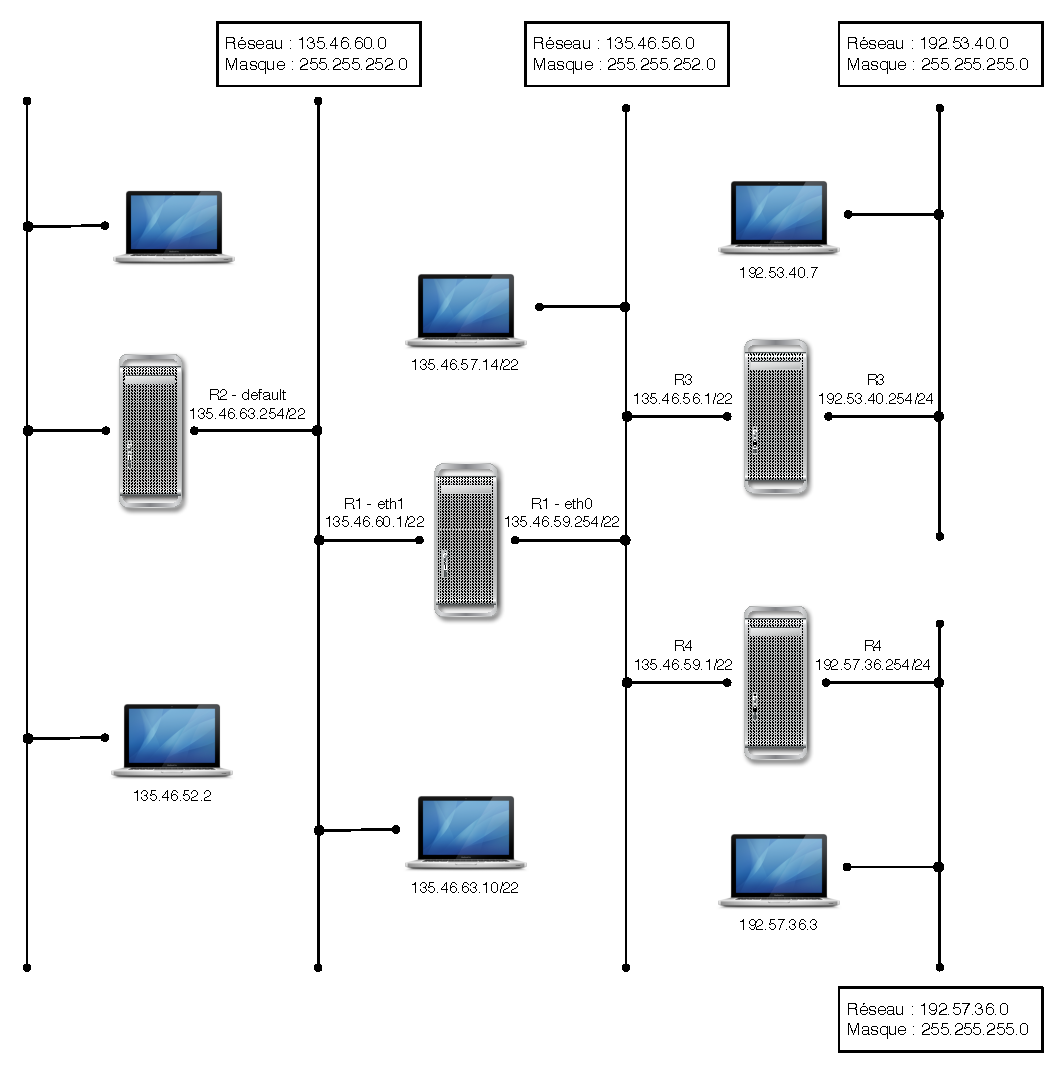
\includegraphics[scale=.7]{Exam2009/reseau-local}
	\end{figure}
\end{ques}

\begin{ques}
	Un routeur peut détruire un datagramme s'il y a congestion et que la file d'attente est remplie. Ou encore si le checksum associé au datagramme n'est pas correct.
\end{ques}

\section{TCP} % (fold)

\begin{ques}
	Etablissement de la connexion s'effectue par un échange de trois messages (\emph{Three way handshake}) afin d'ouvrir la connexion dans les deux sens :
	\begin{figure}[h]
		\center
		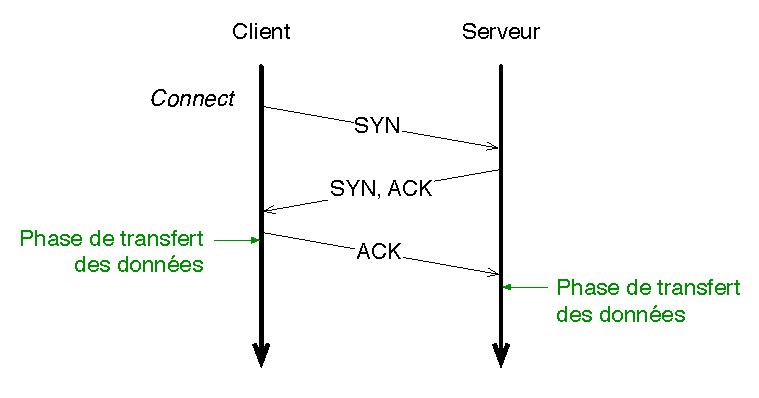
\includegraphics[scale=.7]{../graphes/TCP/Etablissement2}
	\end{figure}
	
	En effet, une connexion TCP qui s'effectuerait par un échange de seulement deux messages n'est pas suffisant :
	\begin{figure}[h]
		\center
		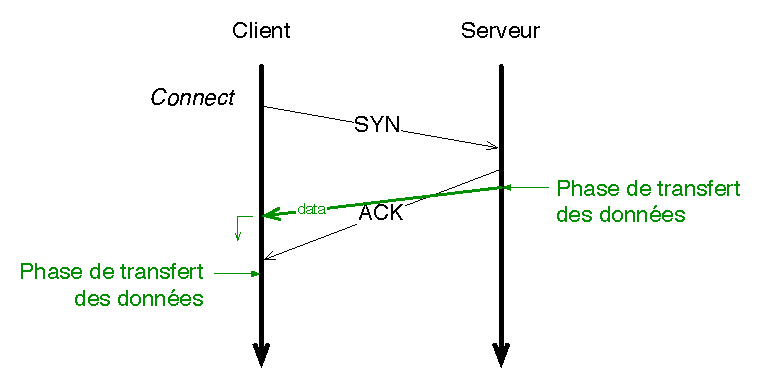
\includegraphics[scale=.7]{../graphes/TCP/Etablissement3}
	\end{figure}
	Puisque les paquets IP dans lesquels sont encpasulés les messages TCP sont des datagrammes, ils sont routés indépendamment les uns des autres. Ainsi, le segment TCP \lstinline!ACK! peut arriver au destinataire après un segment TCP de données (\emph{data}) envoyé par cette même source. Il faut alors un autre message \lstinline!ACK! du destinataire à la source.
\end{ques}

\begin{ques}
	Dimmensionnement du temporisateur de retransmission d'une connexion TCP.\\
	Valeur de $\alpha = 0,85$. Valeur du SRTT (\emph{Smoothed Round Trip Time}) selon la formule : 
	\[SRTT(i+1) = \alpha\times SRTT(i) + (1-\alpha)\times RTT(i)\]
	Considérons $SRTT(0) = 200$ ms. On a alors : \begin{itemize}
		\item $SRTT(1) = 0,85\times 200 + (1-0,85)\times 250=207,5$ ms
		\item $SRTT(2) = 0,85\times 207,5 + (1-0,85)\times 300=221,375$ ms
		\item $SRTT(3) = 0,85\times 221,375 + (1-0,85)\times 350=240,67$ ms
		\item $SRTT(4) = 0,85\times 240,67 + (1-0,85)\times 400=264,57$ ms
	\end{itemize}
\end{ques}

\begin{ques}
	On considère maintenant $\alpha = 0,15$. On a alors :\begin{itemize}
		\item $SRTT(0) = 200$ ms
		\item $SRTT(1) = 0,15\times 200 + (1-0,15)\times 250=242,5$ ms
		\item $SRTT(2) = 0,15\times 242,5 + (1-0,15)\times 300=291,375$ ms
		\item $SRTT(3) = 0,15\times 291,375 + (1-0,15)\times 350=341,21$ ms
		\item $SRTT(4) = 0,15\times 341,21 + (1-0,15)\times 400=391,18$ ms
	\end{itemize}
	
	La valeur $\alpha$ est un facteur de pondération (\emph{smoothing factor}) qui permet de fixer la rapidité à laquelle la nouvelle valeur de SRTT s'adapte aux changements observés. Plus ce facteur $\alpha$ se rapproche de 1, plus les changements de valeur de SRTT seront faibles. A l'inverse, plus $\alpha$ se rapproche de 0, plus les changements de RTT sont pris en compte rapidement dans l'estimation du SRTT.
\end{ques}

\begin{ques}
	TCP évite de mesurer le RTT des segments retransmis. En effet, si TCP prenait en compte les RTT de segments retransmis, les acquittements (\lstinline!ACK!) des transmissions précédentes peuvent être reçus après la retransmission, faussant ainsi la valeur du RTT et celle du RTO (\emph{Retransmission TimeOut}). Cette réduction du RTO augmente la probabilité qu'un segment soit acquitté juste après la retransmission de ce dernier. De ce fait, ces retransmissions non nécessaires gâchent de la bande passante du réseau et diminuent les performances du réseau.
\end{ques}

\section{Codage / décodage} % (fold)

Lors d'un échange capturé sur un réseau local par un analyseur, la trame Ethernet suivante (donnée en hexadécimal, sans préambule, sans CRC) a été observée.

\begin{ques}
	Décodage de la trame.
	\begin{figure}[h]
		\center
		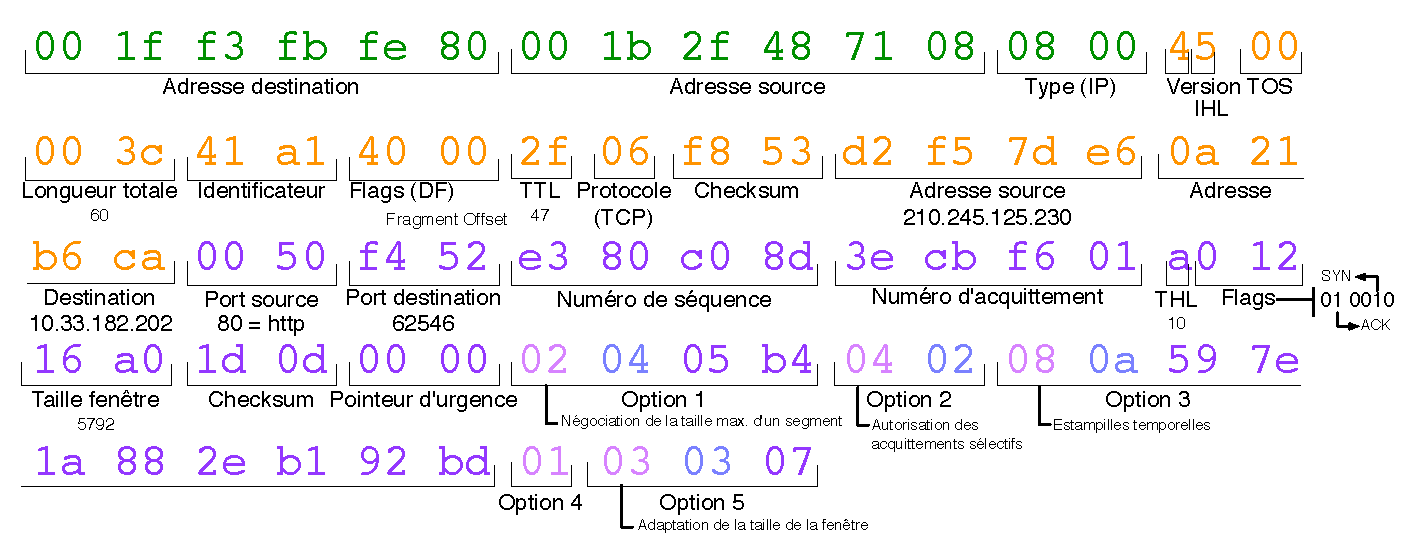
\includegraphics[scale=.7]{Exam2009/trame}
	\end{figure}
\end{ques}

\begin{ques}
	Schéma des différentes machines impliquées : 
	\begin{figure}[h]
		\center
		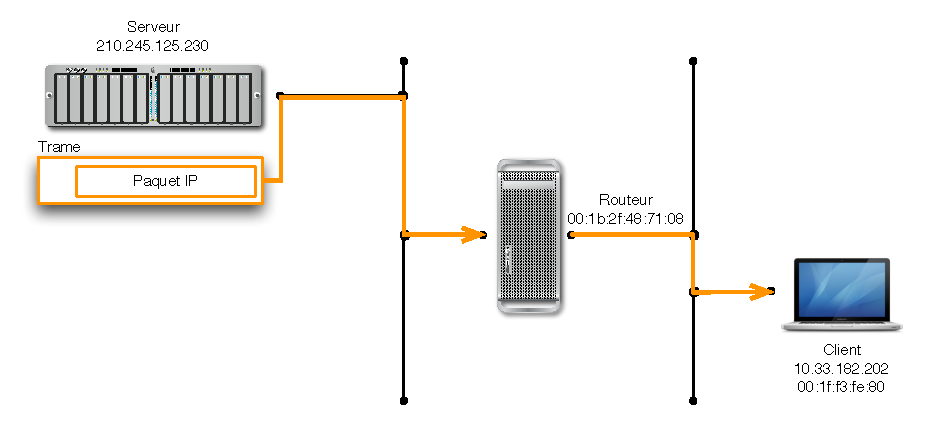
\includegraphics[scale=1]{Exam2009/reseau-local1}
	\end{figure}
\end{ques}

\begin{ques}
	Cette trame contient un paquet IP (type : 0800) reposant sur le protocole TCP (champ \emph{protocol} = 6). Le segment TCP transmis comporte les flags SYN et ACK positionnés à 1 et a comme port source le port 80 (http). On en déduit que c'est la réponse du serveur à la demande de connexion au port 80 du client qui aurait alors effectué une requête ACK.
\end{ques}

\vspace{30pt}

\begin{ques}
	Codage de la trame précédente.
	\begin{figure}[h]
		\center
		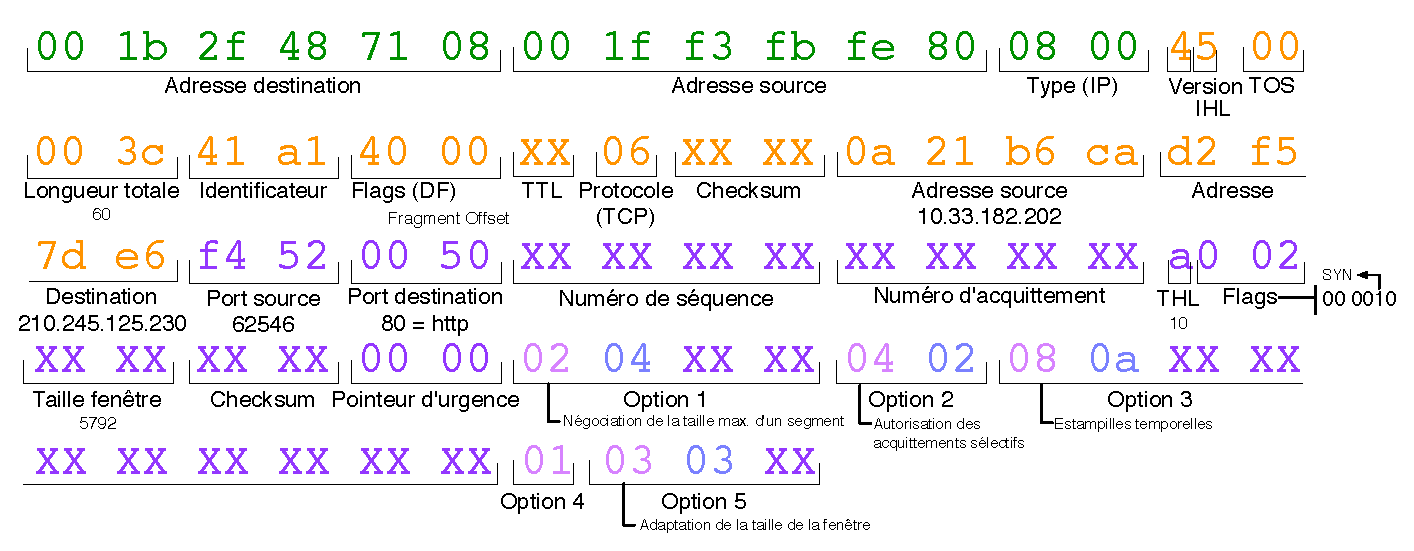
\includegraphics[scale=.7]{Exam2009/trame2}
	\end{figure}
\end{ques}

\end{document}